
L'equazione della quantità di moto è
\begin{equation}
 \rho \left\{ \frac{\partial \bm{u}}{\partial t} +
   \left( \bm{u} \cdot \bm{\nabla} \right) \bm{u} \right\} = 
   \bm{\nabla} \cdot \mathbb{T} + \bm{f}
\end{equation}
dove con $\mathbb{T}$ è stato indicato il tensore degli sforzi,
 che per un fluido newtoniano è $\mathbb{T} = -p \mathbb{I} + \mathbb{S}$
 con $\mathbb{S} = 2 \mu \mathbb{D} + \lambda \left( 
 \bm{\nabla} \cdot \bm{u} \right) \mathbb{I}$ e $\mathbb{D} = \frac{1}{2}
 \left[ \bm{\nabla}\bm{u} + \bm{\nabla}^T \bm{u} \right]$ il tensore
 velocità di deformazione, parte simmetrica del gradiente della velocità.
%
Introducendo la derivata materiale, si ritrova una forma ``familiare''
 del secondo principio della dinamica
\begin{equation}
 \rho\frac{D\bm{u}}{D t} = \bm{\nabla} \cdot \mathbb{T} + \bm{f}
  \qquad \Rightarrow \qquad
 \rho\bm{a} = \bm{\nabla} \cdot \mathbb{T} + \bm{f}
\end{equation}
%
\paragraph{Richiami di geometria delle curve nello spazio.}
Una curva è un luogo di punti che può essere parametrizzato tramite un
 parametro solo.
La parametrizzazione $\bm{r}(t)$ della curva $\bm{r}$ è definita regolare 
 se $d\bm{r}/dt \ne 0$. Si definisce poi una parametrizzazione regolare
 particolare, l'ascissa curvilinea $s$ tale per cui $\left| d\bm{r}(s)/ds
 \right| = 1, \forall s \in (a,b)$.

\noindent 
Nel seguito si introduce brevemente la \textbf{terna di Frenet} 
 $\left\{\bm{\hat{t}}, \bm{\hat{n}}, \bm{\hat{b}} \right\}$, formata
 dai versori tangente, normale e binormale, in funzione dell'ascissa
 curvilinea.
%
Si dimostra che
\begin{equation}
 \bm{\hat{t}}(s) = \dfrac{d\bm{r}}{ds}
\end{equation}
%
La derivata seconda della posizione $\bm{r}$, cioè la derivata prima del
 versore tangente $\bm{\hat{t}}$ è legata al versore normale
 $\bm{\hat{t}}$, tramite la curvatura $k = \left| \frac{d\bm{\hat{t}}}{
 ds} \right|$.
\begin{equation}
 \bm{\hat{n}} = \dfrac{\frac{d\bm{\hat{t}}}{ds}}
    {\left|\frac{d\bm{\hat{t}}}{ds} \right|} 
  \qquad \Rightarrow \qquad
 \dfrac{d\bm{\hat{t}}}{ds} = k \bm{\hat{n}}
\end{equation}
%
Il versore binormale è definito a completare la terna ortonormale 
 destrorsa
\begin{equation}
 \bm{\hat{b}} = \bm{\hat{t}} \times \bm{\hat{n}} 
\end{equation}
%
Per completezza e senza troppo sforzo si calcolano anche le derivate 
 di tali versori, ricordando che hanno modulo unitario e costante,
 e formano una terna ortogonale in ogni punto, introducendo la definizione
 della torsione $\tau = \frac{d \bm{\hat{n}}}{ds}\cdot \bm{b}$.
\begin{equation}
\begin{aligned}
& \qquad \qquad \qquad \qquad \qquad \qquad \qquad \qquad 
  \qquad \qquad \qquad \qquad \quad
 \frac{d \bm{\hat{t}}}{ds} = k \bm{\hat{n}} \\
& \begin{cases}
 \bm{\hat{n}}'\cdot \bm{\hat{n}} = 0 \\
 \bm{\hat{n}}'\cdot \bm{\hat{t}}+\bm{\hat{t}}'\cdot \bm{\hat{n}} = 0 \\
 \bm{\hat{n}}'\cdot \bm{\hat{b}} = \tau \\
 \end{cases} \Rightarrow \quad
 \begin{cases}
 \bm{\hat{n}}'\cdot \bm{\hat{n}} = 0   \\
 \bm{\hat{n}}'\cdot \bm{\hat{t}} = -k  \\
 \bm{\hat{n}}'\cdot \bm{\hat{b}} = \tau \\
 \end{cases} \qquad \quad \quad \Rightarrow \quad 
  \frac{d \bm{\hat{n}}}{ds} = - k \bm{\hat{t}} + \tau \bm{\hat{b}} \\
& \begin{cases}
 \bm{\hat{b}}'\cdot \bm{\hat{b}} = 0 \\
 \bm{\hat{b}}'\cdot \bm{\hat{t}} + \bm{\hat{t}}'\cdot \bm{\hat{b}} = 0 \\
 \bm{\hat{b}}'\cdot \bm{\hat{n}} + \bm{\hat{n}}'\cdot \bm{\hat{b}} = 0 \\
 \end{cases} \Rightarrow \quad
 \begin{cases}
 \bm{\hat{b}}'\cdot \bm{\hat{b}} = 0 \\
 \bm{\hat{b}}'\cdot \bm{\hat{t}} = -\bm{\hat{t}}'\cdot \bm{\hat{b}} = 0 \\
 \bm{\hat{b}}'\cdot \bm{\hat{n}} = -\bm{\hat{n}}'\cdot \bm{\hat{b}} = -k\\
 \end{cases} \Rightarrow \quad
  \frac{d \bm{\hat{b}}}{ds} = - \tau \bm{\hat{n}} \\
\end{aligned}
\end{equation}
%
Se la parametrizzazione regolare della curva non è l'ascissa curvilinea,
 si può ricavare
\begin{equation}
 \frac{d\bm{r}}{dt} = \frac{ds}{dt}\frac{d\bm{r}}{ds} = 
  v \bm{\hat{t}}
\end{equation}
dove si è introdotto il modulo $v$ di quella che sarà la velocità $\bm{v}$
 quando $\bm{r}$ e $t$ saranno spazio e tempo.
In maniera analoga
\begin{equation}
 \frac{d\bm{\hat{t}}}{dt} = \frac{ds}{dt}\frac{d\bm{\hat{t}}}{ds} = 
  v k \bm{\hat{n}}
\end{equation}
 %
Se $\bm{r}$ e $t$ sono spazio e tempo, la velocità e l'accelerazione di un
 punto che ha come legge oraria $\bm{r}(t)$ sono
\begin{equation}
 \begin{aligned}
  \bm{v} & = \frac{d\bm{r}}{dt} = \frac{ds}{dt}\frac{d\bm{r}}{ds} = 
    v \bm{\hat{t}} \\
  \bm{a} & = \frac{d\bm{v}}{dt} =
   \frac{dv}{dt} \bm{\hat{t}} + v \frac{d\bm{\hat{t}}}{dt} =
   \frac{dv}{dt} \bm{\hat{t}} + v^2 k \bm{\hat{n}}
 \end{aligned}
\end{equation}
%
\begin{minipage}{0.60\textwidth}
\paragraph{Ritorno al bilancio della quantità di moto.} Inserendo la
 forma dell'accelerazione nell'equazione della quantità di moto e 
 proiettando lungo i versori della terna di Frenet
\begin{equation}
 \begin{cases}
  \rho \frac{dv}{dt} =  \bm{\hat{t}} \cdot \left(
     \bm{\nabla} \cdot \mathbb{T} + \bm{f} \right) \\
  \rho v^2 k = \bm{\hat{n}} \cdot \left(
     \bm{\nabla} \cdot \mathbb{T} + \bm{f} \right) \\
  0 = \bm{\hat{b}} \cdot \left(
     \bm{\nabla} \cdot \mathbb{T} + \bm{f} \right) \\
 \end{cases}
\end{equation}
In assenza di forze di volume ($\bm{f}=0$) e sforzi viscosi
($\mathbb{T}=\mathbb{S}-p\mathbb{I}=-p\mathbb{I}$):
\begin{equation}
 \begin{cases}
  \rho \frac{dv}{dt} = - \bm{\hat{t}} \cdot \bm{\nabla} p \\
  \rho v^2 k         = - \bm{\hat{n}} \cdot \bm{\nabla} p \\
  0                  = - \bm{\hat{b}} \cdot \bm{\nabla} p \\
 \end{cases}
\end{equation}
\end{minipage}
\hfill
\begin{minipage}{0.40\textwidth}
\begin{center}
   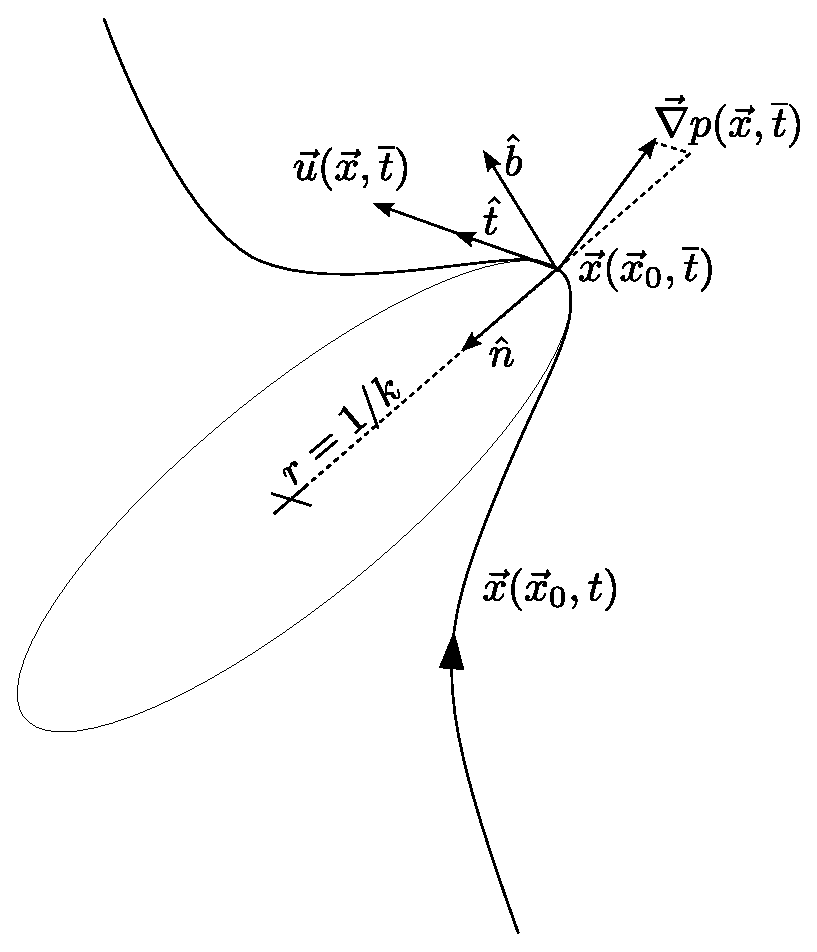
\includegraphics[width=1.0\textwidth]{./fig/frenet.eps}
\end{center}
\end{minipage}
%
Un'analisi della componente normale permette di ricavare, \textbf{sotto le
 ipotesi fatte}, il legame tra la curvatura delle traiettorie delle
 particelle fluide e il gradiente del campo di pressione.
Il termine a sinistra dell'uguale è positivo poichè prodotto di quantità
 positive: la curvatura di una linea è non negativa per come è definita, la
 densità è positiva, il modulo di un vettore è anch'esso non negativo.
Il prodotto scalare tra la normale e il gradiente della pressione
 (derivata direzionale della pressione in direzione $\bm{\hat{n}}$) deve
 quindi essere negativo. La pressione quindi diminuisce, andando verso
 il centro del cerchio osculatore.
Sempre dalla seconda equazione è immediato notare che il legame tra la
 curvatura della traiettoria è proporzionale alla componente del gradiente
 di pressione lungo il versore normale. La componente tangente fa aumentare 
 il modulo della velocità, mentre la componente binormale deve essere nulla.
%Essendo il versore $\bm{\hat{n}}$ diretto verso il centro del cerchio
% osculatore (in parole povere è diretta verso l'interno della curva),
% la curvatura $k$ positiva, segue che la pressione deve diminuire lungo 
% $\bm{\hat{n}}$, cioè aumenta all'allontanarsi dal cerchio del centro
% osculatore (in parole altrettanto povere, ``verso l'esterno'').
%\textit{(Nemmeno a dirlo, la densità $\rho$ è positiva e il quadrato
%  del modulo della velocità $v^2$ è positivo.)}
%\noindent
%Dalla componente lungo $\bm{\hat{n}}$ si nota che il legame tra 
% la componente del gradiente della pressione in quella direzione è
% \textbf{proporzionale} alla curvatura della traiettoria della particella
% fluida.

